\documentclass[a4paper]{article} % gebruik acm style voor je scriptie: [format=acmsmall, screen=true, review=false]{acmart} 
\usepackage{amsmath}
\usepackage{amsfonts}
\usepackage{amssymb}
\usepackage{hyperref}
\usepackage{pdfpages} % http://mirror.unl.edu/ctan/macros/latex/contrib/pdfpages/pdfpages.pdf
\usepackage{booktabs} 
\usepackage{bookmark}
\usepackage{tabularx}

\usepackage[utf8]{inputenc}
\usepackage{amsmath}
\usepackage{graphicx}
\usepackage[colorinlistoftodos]{todonotes} % handig voor commentaar: gebruik \todo{}, zie ftp://ftp.fu-berlin.de/tex/CTAN/macros/latex/contrib/todonotes/todonotes.pdf
\usepackage{listings}
\usepackage{pdfpages}
\usepackage{tcolorbox}
\usepackage{float}
\usepackage{caption}
\usepackage{subcaption}
\usepackage{apacite}
\usepackage{stackengine}
\usepackage{lineno}

\begin{document}
\linenumbers

%\input{titlepage}
\begin{titlepage}


\begin{center}
\textsc{\Large Classifying Dutch municaplity documents using questions from parliament}\\
\textsc{A comparative study on the domain adaptivity of Convolutional Neural Networks, Support Vector Machines, Random Forest and Par2Vec  }

\bigskip

\textsc{\large
submitted in partial fulfillment for the degree of master of science\\
%
\bigskip
Axel Hirschel\\
%
10656146\\
%
\bigskip
master information studies\\
%
data science \\
%
faculty of science\\
%
university of Amsterdam\\
%
\bigskip
2018-06-21
}

\end{center}
 

\vfill

% In case of an internal project, remove External Supervisor or if you had two internal supervisors, change the header into 
%  & First Supervisor & Second Supervisor  \\
\begin{center}
\begin{tabular}{|l||ll|}
\hline
 & \textbf{Internal  Supervisor} & \textbf{External   Supervisor}  \\   
 \hline
\textbf{Title, Name} & Dr Maarten Marx& Tom Kunzler  \\
\textbf{Affiliation} &UvA, FNWI, IvI & Open State Foundation \\ 
\textbf{Email} & maartenmarx@uva.nl&tom@openstate.eu \\
\hline
\end{tabular}
\end{center}


\bigskip

% logos
\begin{center}
\mbox{
\includegraphics[width=.2\paperwidth]{TitlePages/logos/logo-uva.png} 

\includegraphics[width=.2\paperwidth]{TitlePages/logos/ads.png}
\includegraphics[width=.2\paperwidth]{TitlePages/logos/osf.png} % replace by the logo of your internship company or remove
}
\end{center}
\end{titlepage}

  % or use another template

\pagebreak

\tableofcontents

\pagebreak

\begin{abstract}
% [CHANGE] 
\end{abstract}


\section*{Thesis requirements}
\begin{itemize}
\item Your thesis is written in ACM style with two columns  (\texttt{documentclass[sigconf]{acmart}}).
\item It is maximally 10 pages long, excluding the title page and the appendix, but including references, figures, etc 
\end{itemize}


\pagebreak


% Here you input all your sections in seperate files

\section{Introduction}
\label{sec:intro}
Text classification is considered as one of the most important challenges within natural language processing. Classifying documents is vital, as it enables users to easily query and retrieve useful information. Moreover, it allows the automization of many processes such as spam classification and sentiment analysis. Given the wide variety of application, many algorithms have been developed to tackle the problem \cite{aggarwal2012survey}.\\
Bayesian Classifiers are considered a class of classification algorithms, and they classify document based on word occurences within documents. This word presence is used to calculate the probality that certain documents are part of a topic. The two prominent versions of bayesian classifiers are multi-variate Bernoulli models and multinomial models. Another widely used class of text classificatiers are support vector machines (SVM). Within SVM the algorithm creates linear hyperplanes which split the data into classes based on a bag-of-words representation of texts. Using kernel tricks hyperplanes can be constructed which can find more compex relations than linear  \cite{aggarwal2012survey}.\\
Recently, deep neural networks have been employed on classification problems as well. Most notably convolutional neural nets (CNN) have outperformed other methods on baseline classification problems. CNN have been generaly been used on image data, but research in word and document embedding spaces such as Word2Vec \cite{mikolov2013efficient} and Paragraph2Vec \cite{le2014distributed} allow the use of CNN on text as well. Transforming words within documents into a multi-dimensional vectors allows the use of convolutional filters, which shift over the documents and detect patterns within documents \cite{kim2014convolutional}.\\
In contrast to many of the baseline challenges within text classification, real-world application of classification often involves other challenges as well. Within this research documents of Dutch municipalities are classified, which is a difficult task due to three properties. Firstly, no labelled training data is available, which means that training needs to be done on data from the central document. Secondly, many of the documents are multi-topic and it is interesting to discuss how well algorithms deal with this. Thirdly, within classes a large variety of documents exist, as the documents differ in length and style. The research question and subquestions are thus:\\
\begin{itemize}
\item How well does CNN perform on classifying Dutch municipality documents compared to SVM and Bayesian Classifiers? 
\begin{itemize}
\item How does the detail of topics influence the performances of all algorithms?
\item What thresholds are optimal in detecting topics of multi-labeled documents.
\item How well do the performances of the algorithms on the dataset of the central government generalize to the dataset of the municipalities?
\item How can all algorithms be optimized to deal with the large in-class variety of the topics?
\item What are the characteristics of misclassified documents?
\end{itemize}
\end{itemize}
Within the next chapter, the literature review, current approaches to the mentioned challenges and the general idea behind the algorithms is further explained. Then the specific set-up for this research is discussed within the methodology, which also provides information on how the research questions are answered. The results of this research is described next, and provides a detailed overview of the performance of all algorithms with various evaluation metrics. Lastly, the answers to the research questions are formulated and the conclusions from this article are discussed.

%\begin{itemize}
%\item Bevat je onderzoeksvraag (of vragen)
%\item Plaatst je vraag in de bestaande literatuur.
%\end{itemize}
%
%Je onderzoeksvraag is leidend voor je hele scriptie. Alles wat je doet moet uiteindelijk terug te voeren zijn op 1 doel: het beantwoorden van die vraag. 
%
%Typisch zal je het dan ook zo doen:
%
%Mijn onderzoeksvraag is onderverdeeld in de volgende deelvragen:
%
%\begin{description}
%\item[RQ1] \ldots We   beantwoorden deze vraag  door het volgende te doen/ antwoord op de volgende vragen te vinden/ \ldots
%\begin{enumerate}
%\item Vragen op dit niveau kan je echt beantwoorden, en dat doe je in je Evaluatie sectie\ref{sec:eva}.
%\end{enumerate}
%\item[RQ2] \ldots
%\item[RQ3] \ldots
%\end{description}
%%
%Je Evaluatie sectie \ref{sec:eva} bevat evenveel subsecties als je deelvragen hebt. En in elke sectie beantwoord je dan die deelvraag met behulp van de vragen op het onderste niveau.
%
%In je conclusies kan je dan je hoofdvraag gaan beantwoorden op basis van al het eerder vergaarde bewijs.
%
%
%\paragraph{Overview of thesis}
%Hier geef je even kort weer wat in elke sectie staat.
\section{Related Work}
\label{sec:rel}
Classifcation has been a widely studied information problem and its various solutions are discussed within this section. The goal of classification is to assign labels to documents based on its contents. Depending on the task, this is either a binary classification or a multiclass classification problem. This research focusses on multiclass classification and even more specifically, multi-label classification. This means that documents can have multiple labels instead of merely one.\\
All classification is contingent on labeled train data, which is used to train a classifier in distinquishing between various classes. This means that classification of new documents is based on previous experience on other data. Often, a number of pre-processing steps are executed, in order to engineer a document representation which contains relevant content. A common representation is the bag-of-words representation, which is used to transform documents into a vector which indicates how many times words of the vocabulary occur within the text.\\
One of the algorithms that uses bag-of-words as input is the miltinominal naive bayes classifier, which uses probabilities of words occuring within a specific topic in order to classify unseen documents. One of the ways to increase performance is to extend the probabilities based on word occurences with other features, such as which organization published a document or on what kind of domain names documents were found \cite{sahami1998bayesian}. Another version, very similar to Naive Bayes, includes document frequency within the bag-of-words vector, and thus divide the word-occurences within that specific document by the amount of documents in which that word occurs \cite{joachims1996probabilistic}. \\
Another frequently used algorithm for text classification is decision tree, which is an algorithm which establishes a hierarcal division based on textual features. These splits are based on features spaces which have a more skewed distribution of the classes, for example document in which certain words occur are often from a certain class. Multiple trees can be created as an ensemble, each on part of the data, to prevent overfitting to the train data and these are called random forest classifiers. Although the algorithm and its outcome are easily understandable its performance is often worse than other methods \cite{li1998classification}.\\
The last method based on the bag-of-words implementation is the SVM, which has been the state-of-the-art for many years. Within SVM hyperplanes are constructed that split datapoints within the multidimensional space. It is argued that SVM can perform well on textual data, since few features are relevant though those which are relevant correlate. This allows SVM classifiers to easily distinquish between various classes \cite{joachims2001statistical}.\\
All these algorithms based on bag-of-words have had specific classification problems in which they have excelled. However, the bag-of-words representation has a number of detriments. Foremost, the representation is unable to see the relation between "strong" and "powerful". The words are equally far apart as any random word such as "flower". Moreover, the representation treats documents as a collection of words instead of an ordered sequence. These two problems refrain algorithms to identify specific patterns and nuances in texts.\\
Recently, new document representations have been developed which use word embeddings. Word embeddings are multi-dimensional vectors that represent the semantical meaning of words. These embeddings are created using a neighbourhood approach, and therefore words that appear in similar contexts also are located closeby within the multi-dimensional space. \cite{mikolov2013efficient} Documents can then be represented by ordering these word-vectors in the same sequence as original sentences.\\
This representation allows successful employment of neural networks for text classification, and two distinct types can be distinquished: Convolutional Neural Networks (CNN) and Recurrent Neural Networks (RNN). Although both types have achieved state-of-the-art results within various natural language processing tasks, CNN is expected to have better performance on classification tasks where pattern recognition is vital \cite{yin2017comparative}. Moreover, CNN can be trained faster than RNN, because it can be parallized on the GPU. Since keyphrases and similar structures seem to be important for this specific task, and because computational speed is important, CNN have been further explored.\\ 
CNN employ filters that are applied to local features and this has originally been used for processing image data. However, recent research has shown that CNN can also be used for natural language processing tasks. Kim et al. (2014) show that a CNN with Word2Vec-embeddings achieves excellent results, which suggests that the embeddings are good feature extractors. Their architecture consist of multiple pooling layers and 1D-convolutional layers and then two fully connected layers which produce the final output. They also experiment with multiple filter sizes in the convolutional layers, which also increases performance. Their last finding is that dynamically adjusting the embeddings boosts performance in many tasks.\\
CNN are limited to processing sentences with the same length, and most research solves this problem with padding and splitting sentences. This means that a fixed length is chosen as parameter, and sentences that are longer are cut off at that point. Empty vectors are padded to shorter sentences in order to reach the fixed length \cite{kim2014convolutional}  \cite{zhang2015sensitivity}. 
Another approach to deal with different sentence length is the Dynamic Convolutional Neural Network, which allows different sentence-sizes as input. After convolution layers a dynamic k-max-pooling layer, which computes the amount of features pooled to the next layerly based on the sentence's length. Only within the last pooling layer a fixed number of features is pooled and used within the last dense activation layer \cite{kalchbrenner2014convolutional}. This architecture is only suitable for sentences but has been extendend to entire documents as well. This algorithm uses the output from the last layer of the Dynamic Convolutional Neural Network employed on each sentence. Then based on the length of the document these features are then once again used in a Dynamic Convolutional Neural Network \cite{denil2014modelling}. 
Domain adaptation.....................\\



%\subsection{Document representation}
%Documents can be represented in multiple ways when used within text classification. One of these methods is bag-of-words, which means that each document is represented as a vector with the length of the vocabulary. Each entry in that vector represents how many times the corresponding word occurs within that document. \cite{harris1954distributional} Often, this representation is expanded upon with TF-IDF, which includes the inverse document frequency of words as well. Therefore the occurences of words within are scaled based on the total amount of documents in which that word occurs.\\
%A similar representation technique is to represent documents with vectors with a length of the vocabulary size. Within this representation each entry within such a vector is a binary number representing the presence or absence of that word within a document. \\  
%While bag-of-words and these binary vectors have been the standard representation for many years, they do have significant disadvantages. This is foremost caused by the loss of word order within those representations. Also, words with similar meaning, such as "hate" and "loathe" are equally far apart within this representation as words with totally different meaning such as "hate" and "love". This means that this representation is less well equiped to deal with nuanced differences in meaning and context.\\
%Representing documents can also be done using word embeddings. Word embeddings are multi-dimensional vectors that represent the semantical meaning of words. These embeddings are created using a neighbourhood approach, and therefore words that appear in similar contexts also are located closeby within the multi-dimensional space. \cite{mikolov2013efficient} Documents can then be represented by ordering these word-vectors in the same sequence as original sentences.\\
%Using embedding spaces such as Word2Vec are thus not prone to the loss of word order. This means that with these representation also contextual nuances within sentences caused by word order can be understood. This is not possible using only words or bag-of-words, as it is unlikely that specific words occur in the same order within multiple documents.  Moreover, similar sentences are represented by closely related vectors, which allows systems to also understand sentences when other words are used. \\
%PAR2VEC
%
%\subsection{Classifiers}
%\subsubsection{Probalistic models}
%One of the most prominent ways for text classification is the Naive Bayes classifier. The Naive Bayes classifier learns the probability words occur within a certain topic. New documents can be classified using the distribution of words within that document. However, the Naive Bayes assumes that items occur independently of each other, and this assumption often does not hold. Still, the Naive Bayes can perform relatively well. \cite{allahyari2017brief} Two distinct ways of Naive Bayes can be found: Multi-variate Bernoulli model and multinomial model. The main difference is the input for the model. Within the multi-variate Bernoulli the binary vector representation is used and within the multinominal model the bag-of-words is used.\\
%For both models its learning process is relatively similar. For each word it is calculated how many times it occurs in each class. Then this number plus one is divided by the amount of unique words plus the amount of words within documents of that class. This function yields the probability of a document containing that word belongs to a certain class. To classify new documents the probabilities for the words within that document can be calculated. Using these probabilities the relative relative probability of the document to belong to a certain class can be calculated. \cite{mccallum1998comparison}\\
%Although Naive Bayes algorithms are performing quite well they do have some performance issues. It suffers from the problems of the binary and bag-of-words representation. Moreover, the independency assumption also prevents naive bayes from discovering more complex relations within texts, as it is unable to see that co-occurences of specific words can actually define the class of a sentence. \\ 
% 
%\subsubsection{Decision trees}
%Tree-based classifiers classify documents by creating a set of rules based on the presence and absence of words within documents. The training of decision trees is done by splitting the training set into multiple splits. Each individual split is based on the information gain provided, which means that by selecting on the specific feature of this split the greatest amount of extra documents can be classified correctly. To prevent overfitting the data is being split untill each node has a certain minimum of words or untill a maxinum number of splits are performed.
%
%\subsubsection{Linear models}
%\begin{itemize}
%\item SVM classifiers
%
%\item Regression-based classifiers
%
%\end{itemize}
%
%
%\subsubsection{Neural networks}





%Deze sectie bestaat uit een aantal "blokken", waarin je per blok de relevante literatuur beschrijft. 
%
%Neem alleen literatuur op die van belang is voor jouw onderzoeksvraag en deelvragen.
%
%Typisch heb je 1 blok voor je hoofdvraag en per deelvraag \textbf{RQi} een blok. 
%
%
%\subsection{RQ1}
%
%\subsection{RQ2}
\section{Methodology}
\label{sec:meth}
Within this research the final goal is to construct a classifier which is able to classify municipality documents correctly. In order to do this, a multitude of algorithms are examined. Also, the influence of the domain adaptivity and importance sampling are researched. This section introduces the datasets, experiments and further detail about the implementation of the algorithms.

\subsection{Description of the data}
\label{subsec:data}
Two datasets have been used within this research which both include documents from the government of the Netherlands. The first set, called PAR\_ALL, consists of over 50,000 questions and answers that have been asked within the Dutch national parliament during 2001-2017 and these questions were scraped from www.zoek.officielebekendmakingen.nl. The content of these questions and answers ranges from critical examination of proposed laws to requests of more information about ongoing affairs currently within the news. The second set consist of 20,000 documents from Dutch municipalities, such as items on the agenda and notifications of commissions. This set is retrieved with an API of www.zoek.openraadsinformatie.nl and is called MUN\_ALL. \\
Although both sets are political and Dutch, they do vary in content. One of the big differences is that the set of the national government only entails questions with answers, whereas the municipality dataset consist of a greater variety of document types. The themes discussed are also different because within municipalities only local policy is discussed such as the construction of local infrastructure and the re-allocation of local sport clubs. This is in contrast to the parliament, because there broader themes such as criminal law and measure for social security are examined.\\
All of the parliament data is annoted with any number of labels denoting their content. These labels have 2 levels of detail; one broad category such as healthcare or law and one detailed category such as healthcare for the elderly or criminal law. For this research only the 17 broad labels are used, the detailed 118 labels are dropped. The municipality set was not labeled, but for this research manually a part was annotated using the framework of the TaxonomieBeleidsagenda. This taxonomy has also been used to annotate the parliament data. The labeled municipality dataset is named MUN\_LABELED.

\begin{figure}[H]
	\begin{center}
		\includegraphics[width=\linewidth]{"Labels in dataset"}
		\caption{Relative occurences of labels within various datasets}
		\label{fig:distributiontopics}
	\end{center}
\end{figure}

Within Table \ref{sumData} the datasets are summarized, as it shows some characteristics of these sets. Note that for one experiment the dataset with questions of parliaments has been split in two parts, based on when these questions have been asked. The first set consists of all questions from 2001-2009 (PAR\_EARLY) and the second set composed of the questions of 2015-2017 (PAR\_LATE). Figure \ref{fig:distributiontopics} shows the relative occurences of labels within the datasets.

\begin{table}[H]
\caption{Summary of the datasets used within this research}
\label{sumData}
\resizebox{\textwidth}{!}{%
  \begin{tabular}{cccccc}
\footnotesize \textbf{Name Dataset}                     &\footnotesize PAR\_ALL                                                                        &\footnotesize PAR\_EARLY                                                                       &\footnotesize PAR\_LATE                                                                        &\footnotesize MUN\_ALL                                                                                        &\footnotesize MUN\_LABELED                                                                                                                  \\ \midrule
%\textbf{Description}                      & Set of questions and \newline answers asked within the\newline Dutch national parliament\newline between 2001-2017 & Set of questions \newline and answers asked\newline within the Dutch\newline national parliament\newline between 2001-2009 & Set of questions\newline and answers asked\newline within the Dutch \newline national parliament between 2015-2017 & Set of documents\newline such as items on agendas,\newline reports and remarks\newline of a wide variety \newline of Dutch municipalities & Set of documents \newline such as items on agendas, \newline reports and remarks \newline of a wide variety \newline of Dutch municipalities \newline with manually \newline appended labels \\
%\textbf{Retrieved from}                   & zoek.officielebekendmakingen.nl                                                       & zoek.officielebekendmakingen.nl                                                       & zoek.officielebekendmakingen.nl                                                       & zoek.openraadsinformatie.nl                                                                          & zoek.openraadsinformatie.nl                                                                                                        \\
\footnotesize \textbf{Amount samples}                   & \footnotesize 52397                                                                                     & \footnotesize 28063                                                                                     & \footnotesize 8202                                                                                      & \footnotesize 20886                                                                                                    & \footnotesize 439                                                                                                                                    \\
\footnotesize \textbf{Average amount words}             & \footnotesize 688.3                                                                                     &\footnotesize  648.2                                                                                     & \footnotesize 834                                                                                       & \footnotesize 119.4                                                                                                    & \footnotesize 136.8                                                                                                                                  \\
\footnotesize \textbf{Standard deviation words}  &  \footnotesize 429.3                                                                                     & \footnotesize 382                                                                                       & \footnotesize 554.0                                                                                     & \footnotesize 53.2                                                                                                     & \footnotesize 106.8                                                                                                                                  \\
\footnotesize \textbf{Average amount labels}            & \footnotesize 1.62                                                                                      &\footnotesize  1.85                                                                                      & \footnotesize 1.32                                                                                      & \footnotesize -                                                                                              & \footnotesize 1.36                                                                                                                                   \\
\footnotesize \textbf{Standard deviation labels} &\footnotesize  0.76                                                                                      & \footnotesize 0.83                                                                                      & \footnotesize 0.52                                                                                      & \footnotesize - & \footnotesize 0.89                                                                                                                                   \\ \bottomrule
 \end{tabular}}
\end{table}




%Data verzameling en beschrijving van de data

%Hoe is de data verzameld, en hoe heb jij die data verkregen?


%Wat staat er in de data? Niet alleen maar een technisch verhaal, maar ook inhoudelijk. DE lezer moet een goed idee krijgen over de technische inhoud en wat het betekent.
\subsection{Experiments}
The main goal of this research is to correctly classify MUN\_ALL data, but it also examines the effects of the domain shift and domain adaptivity algorithms. The algorithms and their parameters are explained in the next section, as this subsection explains how the research questions are answered. \\
Firstly, it is checked how well the individual algorithms perform on merely the parliament data without any difference between the source and target domain. This means the PAR\_ALL dataset is used and shuffled. Also, around 70 percent of the data is used for training, 15 percent for selecting the best hyper-parameters and 15 percent for the final evaluation. Just like with all the following experiments, the performance of algorithms is based on the micro-average of the F1 score, which balances recall and precision. \\
Secondly, the models are trained on the PAR\_ALL data as source domain and tested on the MUN\_LABELED data. This experiment is done twice per algorithm, as it is executed once with and once without importance sampling. For the importance sampling a logistic regression classifier is used which uses 10,000 samples from PAR\_ALL and all of MUN\_ALL. This classifier is then employed to weigh the remainder of the training data. \\
Thirdly, an experiment very similar to the second experiment is carried out. However, the data is different, because now the source domain is all PAR\_EARLY and the target domain is the parliament data from PAR\_LATE. This experiment is executed to examine how important the domain shift is. 

\subsection{Algorithms}
Within this research newer CNN-classifiers are compared to traditional classifiers such as Support Vector Machines (SVM), Logistic Regression (LR), Random Forest (RF) and Multinominal Naive Bayes (NB). For all these implementations the input is a bag-of-words representation of the various documents. The implementation of Scikit-Learn is employed for these algorithms and the optimal hyper-parameters are chosen based on a grid-search. Moreover, when needed, the one-versus-all classifier is used to make the classifiers multi-class. To ensure multi-label outcomes multiple thresholds for prediction are experimented with.  \\
Instead of bag-of-words CNN uses word embeddings as input.  This research experiments with two embeddings, namely pre-trained embeddings retrieved trained on a variety of Dutch resources \cite{tulkens2016evaluating} and self created embeddings using Word2Vec-implementations from Gensim trained on PAR\_ALL and MUN\_ALL. \\
One of the employed CNN within this research is similar to earlier architectures \cite{kim2014convolutional}. This means that an embedding layer is used to transform sentences to a multi-dimensional space using one of the two Word2Vec-embeddings. Both embedding spaces have been tested with static and non-static initializations which indicates whether the embeddings can alter during training.\\
Thereafter three convolutional layers and three max-pooling layers are alternated between. For the convolutional layers multiple filter sizes have been tested and in addition also multiple filter sizes in one layer are experimented with. Then the multidimensional is flattened and a dropout layer is used to prevent overfitting within the network. In some architectures also L1-regularization has been used, however, later research demonstrated the minimal effect of this regularization \cite{zhang2015sensitivity}. \\
The last two layers are fully connected layers in order to gain the final prediction. Since the classification task is multilabel, binary crossentropy is used as loss function in combination with the sigmoid function as activation within the final dense layer \cite{nam2014large} \cite{Multiclass}. The output of the sigmoid function is a number between 0 and 1 per label, and multiple thresholds are tested in order to determine when to predict a certain label. All the parameters of this standard version of CNN are listed in Table \ref{ParametersCNN}\\

\begin{table}[H]
\centering
\caption{Parameter and values within standard CNN}
\label{ParametersCNN}
\begin{tabular}{@{}ll@{}}
\toprule
\textbf{Parameter}      	& \textbf{Values}                             			\\ \midrule
Word2Vec Model          	& Pre-trained, trained on corpus              		\\
Word2Vec Initialization 	& Dynamic, Static                            			\\
Amount of filters       	& 1,3                                        				\\
Filter sizes with one filter 	& 3,5,7,11						 	\\
Filter sizes with three filters& [2,3,4],[3,4,5],[7,8,9]				 	\\
Threshold of prediction	& 0.3,0.4,0.5,0.6,0.7                         			\\ \bottomrule
\end{tabular}
\end{table}

An addition of this research is a slight variation to Kim's architecture which splits the input into smaller blocks of length 200 instead of choosing a pre-defined length of the input sentences. Training is done on smaller blocks of input and when predicting sentences each of the individual blocks of the sentence are classified individually. These predictions are aggregated into one prediction per sentence, either by summing or using the max value of the predictions per block. Then once again predictions above a certain threshold are predicted to belong to that label, and those below that threshold are considered not to have that label. The parameters for this version are similar to those of the Kim's standard implementation, but all the extra parameters are listed in Table \ref{ParametersCNNSplit}.

\begin{table}[H]
\centering
\caption{Extra parametera and values within CNN-split}
\label{ParametersCNNSplit}
\begin{tabular}{@{}ll@{}}
\toprule
\textbf{Parameter}      	& \textbf{Values}                             			\\ \midrule
Input size              		& 200			                               			\\
Aggregation             	& sum, max                                    			\\
\end{tabular}
\end{table}


%The data used within this project consist of two types of data, both from the government of the Netherlands. The first set consists of over 50,000 questions with answers that have been asked within the Dutch national parliament. The content of these question ranges from critical examination of proposed laws to requests of more information about ongoing affairs currently within the news.\\ 
%
%\begin{figure}[H]
%	\begin{center}
%		\belowbaseline[0pt]{ 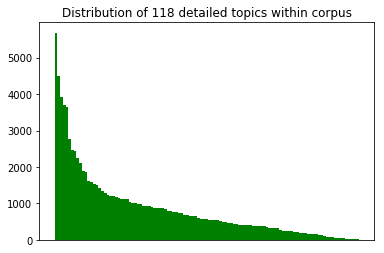
\includegraphics[width=.49\linewidth]{TrainLabels118}}~\belowbaseline[0pt]{ 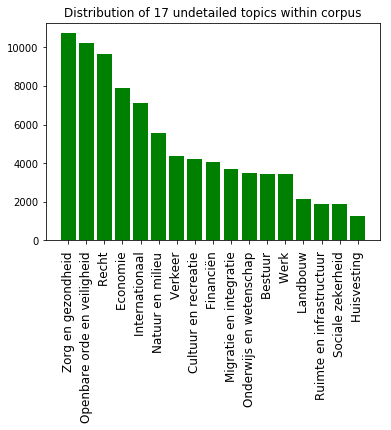
\includegraphics[width=.49\linewidth]{TrainLabels17}}
%		\caption{Distribution of labels within the parlement data}
%		\label{fig:distributiontopics}
%	\end{center}
%\end{figure}
%
%Each question-answer pair is annotated with a number of labels. Each of the labels then consists of two levels of detail; it has one of the 17 undetailed labels, such as law or education, and one of the 118 more detailed labels, such as criminal law or primary education. Figure \ref{fig:distributiontopics} shows the distributions of labels within the dataset and figure \ref{fig:LabelAmount} shows how many labels each document contains.\\
%
%\begin{figure}[H]
%	\centering
%  	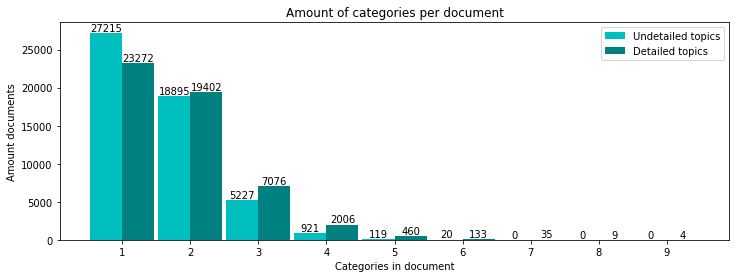
\includegraphics[width=.9\linewidth]{TrainAmountLabels}
%  	\caption{Amount of labels per document}
%  	\label{fig:LabelAmount}
%\end{figure}
%
%The questions are collected from www.zoek.officielebekendmakingen.nl with a scraper and the set consist of all question asked from 2001 to 2017. This means all of the labels have been discussed in many debates and varieties. Moreover, the documents vary on length as can be seen in Figure \ref{fig:WordAmount} and which politicians have asked and answered these questions.\\
%
%\begin{figure}[H]
%	\centering
%  	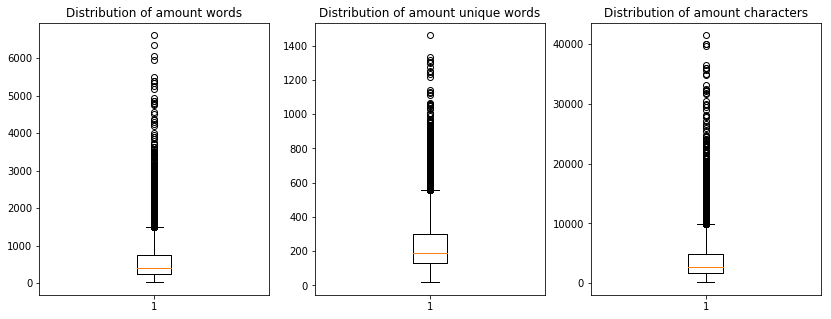
\includegraphics[width=.9\linewidth]{TrainAmountWords}
%  	\caption{Box plots of the amount of words, unique words and characters within the train data.}
%  	\label{fig:WordAmount}
%\end{figure}
%
%The second part of the data is retrieved from www.zoek.openraadsinformatie.nl, which contains documents of Dutch municipalities. These municipality documents consist of all kind of documents produced within municipalities, such as items on the agenda and notifications of commissions. These too have a great variety in content which ranges from discussion about local infrastructure to the re-allocation of local sport clubs. \\

%\begin{figure}[H]
%	\begin{center}
%		\includegraphics[width=.9\linewidth]{MunLabels17}
%		\caption{Distribution of labels within the municipality data}
%		\label{fig:MunLabels17}
%	\end{center}
%\end{figure}
%
%Large amounts of municipality data can be collected, but for this research just 25000 documents were used. Around 500 of these document were manually labeled using the taxonomieBeleidsagenda, which is the same taxonomy used for the Dutch parliament. However, the detailed labels have not been assigned, as these are too specific for untrained annotators. Similar to the training set, an overview of the label distribution, amount of labels and length of the labeled documents are visualized within Figures \ref{MunLabels17},\ref{MunAmountLabels} and \ref{MunAmountWords}. \\

%\begin{figure}[H]
%	\centering
%  	\includegraphics[width=.9\linewidth]{MunAmountLabels}
%  	\caption{Amount of labels per municipality document}
%  	\label{fig:MunAmountLabels}
%\end{figure}
%
%\begin{figure}[H]
%	\centering
%  	\includegraphics[width=.9\linewidth]{MunAmountWords}
%  	\caption{Box plots of the amount of words, unique words and characters within the municipality data.}
%  	\label{fig:MunAmountWords}
%\end{figure}

%This research adds to the existing architectures in its method to deal with variable document sizes instead of merely padding and cutting sentences to the input size. Two possibilities have been examined; Firstly, the sentences are split into multiple smaller parts. Each of these individual parts of the sentence are classified individually. Then these predictions aggregated into one prediction, either by summing or using the max value. Then once again these predictions are rounded per label to create a prediction. All the parameters of the basic version of CNN are listed in Table \ref{ParametersCNN}.\\
%The second implementation attempts to fix the length discrepency within the embedding stage. The documents are all split in an equal number pieces. These pieces are then embedded using the Par2Vec embeddings \cite{le2014distributed}, which employs a pre-trained embedding space. This method ensures that all the documents have an equal input size for the network, however, for some documents the embeddings represent multiple words or even entire paragraphs. Similarly to the other classifiers, multiple parameters are tested such as input-size, static and non-static initialization and filter sizes. \\ 

%\subsection{Experiments}
%The various algorithms are evaluated on the basis of two test-sets, both from a different source of data as explained in section \ref{subsec:data}. The first experiment is carried out on the data with question of the Dutch parlement. This set is split into three parts of respectively 70, 20 and 10 percent of the data. The models are firstly trained on 70 percent of the data. Then, the optimal hyperparameters, such as the decision threshold, are chosen by evaluating the performance on the 20 percent of the data. When these parameters have been selected, the final versions is tested with the last 10 percent of the data. This experiment is conducted twice, using both the data with 17 and 118 different topics. Using different amount of topics shows how well algorithms perform depending on the detail of the topics.\\
%Within the second experiment the transfer between different datasets is specifically important. The model is trained on 80 percent of the parlement-data and the remaining parlement data is used as validation data to select the optimal parameters. However, this model is evaluated using the manually labelled dataset of the Dutch municipalities in order to see how well the models transfer to another dataset. In contrast to the first experiment this experiment is merely conducted with 17 topics, as the municipality data is only classified that way.\\
%Success in both experiments is measured using the micro-average F1-score, which balances the precision and recall of the prediction. However, in addition to the F1-scores also confusion matrices are used in order to evaluate what kind of errors are made. Lastly, properties of documents that are missclassified are evaluated per algorithm to better understand how the algorithms perform on specific types of documents. 


%Hoe je je vraag gaat beantwoorden.
%
%
%Dit is de langste sectie van je scriptie. 
%
%Als iets erg technisch wordt kan je een deel naar de Appendix verplaatsen. 
%
%Probeer er een lopend verhaal van te maken.
%
%Het is heel handig dit ook weer op te delen nav je deelvragen:
%
%\subsubsection{RQ1}
%
%\subsubsection{RQ2}
\section{Evaluation}
\label{sec:eva}

Met een subsectie voor elke deelvraag.

In hoeverre is je vraag beantwoord?

Een mooie graphic/visualisatie is hier heel gewenst.

Hou het kort maar krachtig.
\section{Conclusions}
\label{sec:conc}

Hierin beantwoord je jouw hoofdvraag op basis van het eerder vergaarde bewijs.



\section{Acknowledgements}
I would like to thank everyone from Open State foundation for their support and friendliness during my internship. I have always gone to OSF with great pleasure due to the good political discussions. Moreover, I have greatly appreciated the help of Maarten Marx and Tom Kunzler, as they constantly proposed new ideas and critically looked at mine. Lastly, thanks to my parents Diederik and Moniek, siblings Max and Iris, girlfriend Amber and friends Joppe, Simon, Ethan and Josse for keeping me motivated and supporting me during the entirety of my studies.

% your refs

\bibliographystyle{apacite}
\bibliography{MyThesis}



%\input{appendix}



% Example
%
\includepdf[nup=2x3 , pages=-]{sargent-lecture_slides.pdf}
 
\end{document}
